\documentclass{sigchi-ext}
% Please be sure that you have the dependencies (i.e., additional
% LaTeX packages) to compile this example.
\usepackage[T1]{fontenc}
\usepackage{textcomp}
\usepackage[scaled=.92]{helvet} % for proper fonts
\usepackage{graphicx} % for EPS use the graphics package instead
\usepackage{balance}  % for useful for balancing the last columns
\usepackage{booktabs} % for pretty table rules
%\usepackage{ccicons}  % for Creative Commons citation icons
\usepackage{ragged2e} % for tighter hyphenation
\usepackage{amsmath} % 数式の場合分け用
\usepackage{algorithm,algorithmicx} % 疑似コード用
\usepackage{algpseudocode} % 疑似コード用
%\floatname{algorithm}{Figure}
% Some optional stuff you might like/need.
% \usepackage{marginnote}
% \usepackage[shortlabels]{enumitem}
% \usepackage{paralist}
% \usepackage[utf8]{inputenc} % for a UTF8 editor only

%% EXAMPLE BEGIN -- HOW TO OVERRIDE THE DEFAULT COPYRIGHT STRIP --
\copyrightinfo{
Permission to make digital or hard copies of all or part of this work for personal or classroom use is granted without fee provided that copies are not made or distributed for profit or commercial advantage and that copies bear this notice and the full citation on the first page. Copyrights for components of this work owned by others than ACM must be honored. Abstracting with credit is permitted. To copy otherwise, or republish, to post on servers or to redistribute to lists, requires prior specific permission and/or a fee. Request permissions from Permissions@acm.org. \\
{\sl Ubicomp/ISWC'16 Adjunct}, September 12-16, 2016, Heidelberg, Germany \\
\copyright \ 2016 ACM. ISBN 978-1-4503-4462-3/16/09...\$15.00 \\
DOI: http://dx.doi.org/10.1145/2968219.2968291
}
%% EXAMPLE END


% Paper metadata (use plain text, for PDF inclusion and later
% re-using, if desired).  Use \emtpyauthor xwhen submitting for review
% so you remain anonymous.
\def\plaintitle{A Recognition Method for Continuous Gestures with an Accelerometer}
\def\plainauthor{Hikaru Watanabe, Masahiro Mochizuki, Kazuya Murao, Nobuhiko Nishio}
\def\emptyauthor{}
\def\plainkeywords{Accelerometer, Gesture recognition, Continuous gestures}
\def\plaingeneralterms{Documentation, Standardization}

\title{A Recognition Method for Continuous Gestures with an Accelerometer}

\numberofauthors{4}
% Notice how author names are alternately typesetted to appear ordered
% in 2-column format; i.e., the first 4 autors on the first column and
% the other 4 auhors on the second column. Actually, it's up to you to
% strictly adhere to this author notation.
\author{%
\alignauthor{%
\textbf{Hikaru Watanabe}\\
\affaddr{Graduated School of Information Science and Engineering, Ritsumeikan University} \\
\affaddr{Shiga, Japan} \\
\email{light@ubi.cs.ritsumei.ac.jp} }
\alignauthor{%
\textbf{Kazuya Murao}\\
\affaddr{College of Information Science and Engineering, Ritsumeikan University} \\
\affaddr{Shiga, Japan} \\
\email{murao@cs.ritsumei.ac.jp} }
\vfil \alignauthor{%
\textbf{Masahiro Mochizuki}\\
\affaddr{Research Organization of Science and Technology, Ritsumeikan University}\\
\affaddr{Shiga, Japan} \\
\email{moma@ubi.cs.ritsumei.ac.jp} }
\alignauthor{%
\textbf{Nobuhiko Nishio}\\
\affaddr{College of Information Science and Engineering, Ritsumeikan University} \\
\affaddr{Shiga, Japan} \\
\email{nishio@cs.ritsumei.ac.jp} } }
% Make sure hyperref comes last of your loaded packages, to give it a
% fighting chance of not being over-written, since its job is to
% redefine many LaTeX commands.
\definecolor{linkColor}{RGB}{6,125,233}
\hypersetup{%
pdftitle={\plaintitle},
%  pdfauthor={\plainauthor},
pdfauthor={\emptyauthor},
pdfkeywords={\plainkeywords},
bookmarksnumbered,
pdfstartview={FitH},
colorlinks,
citecolor=black,
filecolor=black,
linkcolor=black,
urlcolor=linkColor,
breaklinks=true,
}

% \reversemarginpar%

\begin{document}
        \maketitle

        % 疑似コード用 ForToの定義
        \algnewcommand\algorithmicto{\textbf{to}}
        \algdef{SE}[FOR]{ForTo}{EndFor}[2]{\algorithmicfor\ #1\ \algorithmicto\ #2\ \algorithmicdo}{\algorithmicend\ \algorithmicfor}%

        % Uncomment to disable hyphenation (not recommended)
        % https://twitter.com/anjirokhan/status/546046683331973120
        \RaggedRight{}

        % Do not change the page size or page settings.
        \begin{abstract}
            Along with the spread of smart phones and wearable devices, systems that recognizes gestures such as punch and chop using an accelerometer have recently been attracting a great deal of attention. However, these systems do not consider the situation that gestures are performed continuously from/to other gestures or untrained movements and can not recognize such gestures accurately. This paper proposes a method that recognizes gestures performed continuously without explicit intervals. The proposed method detects segments similar to template data of target gestures and chooses the most likely segment. In order to evaluate the effectiveness of the proposed method, an experiment is conducted with five subjects. The subjects conducted three types of gestures drawing a graphic symbol in the air; circle, triangle, and cross in five kinds of situations, and ten types of gestures drawing a numeric character in the air; zero to nine. The average F-measure of graphic symbol achieved 0.78 and the average F-measure of numerical character achieved 0.79.
        \end{abstract}

        \keywords{\plainkeywords}

        \category{H.5.m}{Information interfaces and presentation (e.g.,
        HCI)}{Miscellaneous}

        % \section{ACM Copyrights \& Permission}
        % Accepted extended abstracts and papers will be distributed in the
        % Conference Publications. They will also be placed in the ACM Digital
        % Library, where they will remain accessible to thousands of researchers
        % and practitioners worldwide. To view the ACM's copyright and
        % permissions policy, see:
        % \url{http://www.acm.org/publications/policies/copyright_policy}.

        
        \section{Introduction}

        Along with the spread of smart phones and wearable devices, services using activity recognition technologies such as interface, life-log, and supporting system have been proposed, and systems that recognize gestures have recently been attracting a great deal of attention. A gesture recognition system with an accelerometer generally collects acceleration data of the gestures to be recognized (i.e., template data) and calculates the similarity between input acceleration data and each template data, then outputs the label of most similar template data as a result of gesture recognition. With this approach, gestures are recognized with high degree of accuracy only if gestures are clearly segmented, while gestures performed continuously from/to other gestures or untrained movements cannot  be recognized accurately since segmenting gestures is difficult. 
        
        As segmentation methods, users are forced to stand still before and after the gesture or to specify the segment of gestures such as by pushing a button of a wearable device. These methods are not applicable to continuous gestures because there is no clear interval between gestures. Therefore, it is desirable to segment gestures only with acceleration data. 
        
        This paper proposes a method that recognizes gestures performed continuously from/to other gestures or untrained movements with high degree of accuracy. The proposed method detects the segment similar to template data on the fly from input stream of acceleration data. Since multiple templates may find a segment at the same time, the proposed method validates the most similar segment and outputs the gesture label of the segment. 
        % We use SPRING for detecting the segments similar to template data. SPRING is the algorithm to detect a subsequence similar to a template data. However, SPRING has problems that it may miss continuous gestures and do not consider multiple template data.
        % Therefore, we use improved SPRING algorithm to detect gestures.

        \section{Related Work}
        Activities that lasts for a certain time length, such as walking and running are generally segmented with a sliding window and recognized by calculating feature values such as average and variance over the segment, with a classifier such as support vector machine (SVM) and random forest (RF), while gestures are once-off actions that has a starting point and endpoint and have to be segmented with tight-fitting window.
        In addition, gestures to be recognized are similar to each other in many cases. The method using feature values is not suitable for gesture recognition since feature values lose temporal information, therefore, similarity of gestures is calculated with time-series as it is without feature extraction \cite{izuta,uwave}.

        As similarity calculation algorithms, dynamic time warping (DTW) \cite{dtw} and hidden Markov models (HMM) \cite{hmm} are often used. DTW is a method to calculate the distance between two time-series data. HMM is a method to calculate the likelihood of input data to the model made from template data. HMM is often used in speech recognition, however, it requires large amount of template data, therefore DTW is often used in accelerometer-based gesture recognition.

        Izuta et al. \cite{izuta} proposed a method to recognize gestures before the gesture ends. This method improves DTW to calculate the distance between input data stream and template data incrementally and to output the result of gesture recognition when the difference between the shortest distance and the second shortest distance becomes large. However, this study uses test data that have already been segmented and does not consider continuous gestures.
        
        Murao et al. proposed two methods to segment and recognize gestures performed while non-gesture activities. One is a method to classify activities into posture, behavior, and gesture and recognize them individually \cite{murao-const}. Posture is a static activity such as standing and sitting, and behavior is a periodic activity such as walking and running in this work. Specifically, if the variance of the acceleration is low, input data is classified to posture and recognized with SVM that has learned postures only. Otherwise, this method calculates auto-correlation function (ACF) to classify the input data to behavior or gesture. If ACF of acceleration shows high peak, input data is classified to behavior since there is periodic movements and recognized with SVM that has leaned behaviors only, otherwise input data is classified to gesture since there is less periodic movements and recognized with DTW that has learned gestures only. The other one is the method to recognize activities combined with posture, behavior, and gesture \cite{murao-comb}. This method uses five accelerometers on both wrists, hip and both legs. The classification method using ACF in \cite{murao-const} is used to classify activity on each body part. Activities on each body part are recognized individually and integrated into one combined activity. 
        
        The following two works handle both gestures and non-gesture activities.
        Korpela et al. \cite{joseph} proposed a method to recognize both gestures and non-gesture activities with a smartwatch and a smartphone. This method uses random forest and measured power consumption of calculating feature values and DTW distance for each tree. The trickiest part of the work is that low-cost feature set are calculated on the wearable device and high-cost calculations such as DTW are conducted on the smartphone since the wearable device has poorer processor and smaller battery.
        Park et al.\cite{park} proposes a gesture recognition system with a hand-worn sensor and mobile device. This system segments a gesture with a two-stage threshold-based filter with an accelerometer and a gyroscope. A novel point of the paper is to automatically adjust the threshold according to four mobility situations; RIDE, STAND, WALK, and RUN. Then features are extracted from the segment and are recognized with an HMM. The HMM they proposed is a multi-situation HMM, which changes the models according to the mobility situation. However, the models are trained with all combinations of gestures and mobility situations. 
        %However, these method consider the situation that gestures performed from/to still. Therefore
        These methods are able to treat gestures performed before and after other activities without break, however continuously performed gestures without break cannot be segmented and recognized.

        \section{Proposed Method}
        In this paper, we propose a method that recognizes gestures continuously performed from and to other gestures or untrained movements without interval. The proposed method detects the segment that matches a template data in the input stream of acceleration data.
        SPRING algorithm proposed by Sakurai et al. \cite{sakurai} can find segments in various kinds of time-series data, which is an online algorithm to calculate DTW distance and automatically segments input data to match with a template data.
        
        SPRING detects the subsequence in the input stream data that has lower distance to a query of time-series than the predefined threshold. However, SPRING may miss gestures when gestures occurred continuously without an interval since SPRING does not assume that target subsequence appears multiple times without a break. Therefore, we improve SPRING so as to detect such subsequences.
        
        Moreover, SPRING does not accept multiple queries to detect subsequences from input time-series data. Gesture recognition systems are generally configured to recognize multiple kinds of gestures. Simply using SPRING algorithm that detects an individual gesture in parallel would output multiple recognition results at the same time even though a user does not perform multiple gestures at once, therefore the proposed method chooses the best candidate out of the results obtained from each SPRING algorithm.
        
        This section first introduces the classic SPRING algorithm, and explains the improved SPRING algorithm and the gesture selection procedure.

        \subsection{Classic SPRING algorithm}
        \label{sec:spring}

        SPRING is an algorithm to find a segment that is similar to a template data called query from input time-series data. Algorithm \ref{fig:spring-original} shows the algorithm of SPRING. When the input data stream $X=x_{1}, \dots, x_{n}$ whose length is $n$ is being obtained from a sensor and the template data of the gesture to be recognized is $Y=y_{1}, \dots, y_{m}$ whose length is $m$, a derivative template $Y'=y_0, y_1, \dots, y_m$ is defined, where $y_0=(-\infty:+\infty)$ shows zero distance to any values, which is called star padding. Then, an $(m+1)\times n$ matrix ${\bf d}$ is defined by the following equation, where ${\bf d}$ is initialized with ${\bf d}(t,0)=0~(1\leq t\leq m)$ and ${\bf d}(0,i)=\infty~(1\leq i\leq n)$.
        \begin{eqnarray}
            \label{eq:dist-wt}
            {\bf d}(t,i)=| x_{t} - y_{i} |+min\left\{\begin{array}{ll}
            {\bf d}(t-1,i-1) \\
            {\bf d}(t-1,i)\\
            {\bf d}(t,i-1)
            \end{array} \right.
        \end{eqnarray}
           
        \begin{algorithm}[!t]
            \begin{algorithmic}[1]
%                \State{\textbf{Algorithm SPRING}}
                \State{\textbf{input}: $X=\{x_1,\dots,x_n$\}
                \State{\textbf{output}: subsequence matching $Y'=\{y_0,y_1,\dots,y_m\}$}}
                \State{$ d_{min} = \infty $}
                \ForTo{$t = 1$}{$n$}
                \ForTo{$i = 0$}{$m$}
                \State{calc. ${\bf d}(t,i)$ with Eqn. \ref{eq:dist-wt}}
                \State{calc. ${\bf s}(t,i)$ with Eqn. \ref{eq:point-wt}}
                \EndFor
                \If{$d_{min} \leq \varepsilon$}
                \If{$\forall_{i}, {\bf d}(t,i) \geq d_{\min} \cup {\bf s}(t,i) > t_{e} $}
                \State{Report$(d_{\min} , t_{s} , t_{e})$}
                \ForTo{$l=1$}{$m$}
                \If{${\bf s}(t,l) \leq t_e $}
                \State{${\bf d}(t,l) = \infty$}
                \EndIf
                \EndFor
                \EndIf
                \EndIf
                \If{${\bf d}(t,m) \leq \varepsilon \cap {\bf d}(t,m)<d_{min}$}
                \State{$d_{min} = {\bf d}(t,m);~t_s = {\bf s}(t,m);~t_e = t$}
                \EndIf
                \EndFor
                %\State{Substitute $d'_{i}$ for $d_{i}$}
                %\State{Substitute $s'_{i}$ for $s_{i}$}
            \end{algorithmic}
            \caption{SPRING algorithm.}
            \label{fig:spring-original}
        \end{algorithm}
        
        ${\bf d}(t,i)$ is the distance between a template data $Y[1:i]$ and a subsequence in the input time-series $X[t_s:t]$, where $t_s$ is the starting point of the subsequence in the input data that best matches $Y[1:i]$. Therefore the smallest distance $D(X[t_s:t_e],Y)$ is obtained by 
        \begin{equation}
            D(X[t_s:t_e],Y)={\bf d}(t_e,m)=\min({\bf d}(t,m))
        \end{equation}
        where $t_e$ is the endpoint of the subsequence in the input data that best matches $Y[1:m]$. The endpoint $t_e$ is \\$arg\min_t{\bf d}(t,m)$.
        
        However, just by calculating Eqn. \ref{eq:dist-wt}, the starting point $t_s$ cannot be obtained. Therefore, the matrix ${\bf d}(t,i)$ also has information on starting point ${\bf s}(t,i)$ in addition to distance as follows.
        \begin{eqnarray}
            \label{eq:point-wt}
            {\bf s}(t,i) =\left\{\begin{array}{ll}
                {\bf s}(t,i-1) & ({\bf d}(t,i-1) = d_{best} ) \\
                {\bf s}(t-1,i) & ({\bf d}(t-1,i) =  d_{best} ) \\
                {\bf s}(t-1,i-1) & ({\bf d}(t-1,i-1) = d_{best} )
            \end{array} \right.
        \end{eqnarray}
        $d_{best}$ is $\min{\{{\bf d}(t-1,i-1), {\bf d}(t-1,i), {\bf d}(t,i-1)\}}$ in Eqn. \ref{eq:dist-wt}. By calculating Eqn. \ref{eq:dist-wt} and \ref{eq:point-wt}, the best matching subsequence $X[{\bf s}(t_e,m):t_e]$ is found.
        
        %$d(t,i)(t=1,\cdots,n;i=1,\cdots,m) $ is the distance between time-series data and a template data on the point $ (t,i) $, and $ s(t,i) $ is the starting point correspond $ d(t,i) $.
        %Then, $d(t,i) $ and $s(t,i)$ are given by Eqn. \ref{eq:dist-wt} and Eqn. \ref{eq:point-wt}.

        SPRING calculates the distance between the input data $X=\{x_1,\dots,x_t\}$ and a template data $Y=\{y_1,\dots,y_m\}$ and reports the subsequence if the smallest distance so far $d_{min}$ is smaller than threshold $\varepsilon$, and all ${\bf d}(t,i)$ is equal to or larger than $d_{min}$ or all $s(t,i)$ is larger than $t_e$. The last two conditions are employed to avoid multiple subsequences from overlapping afterwards. Then, distance ${\bf d}(t,l)$ is initialized with $\infty$ again if $s(t,l)\leq t_e$ for $l=1$ to $m$. Lastly, the starting point and the endpoint of the subsequence are updated with $t_s=s(t,m)$ and $t_e=t$, respectively. 
        
        Through this procedure, the segment from $x_{t_s}$ to $x_{t_e}$ is found as a subsequence that matches $Y$. 
        %This requirement is to detect the optimal sequence whose distance is smallest. If this requirement is satisfied, it is not possible that the subsequence whose distance is smaller than present one will appear when following time-series data is inputted. 
        However, SPRING may miss out gestures when same gestures are performed continuously without a break. Figure \ref{fig:miss-chop-5x} shows the results of gesture recognition when chop gestures are performed five times without breaks and four out of five trials were correctly detected, however, fourth chop was not detected. SPRING detects a subsequence if $\forall_i, {\bf d}(t,i) \geq d_{min}$ is met at line 10 in Algorithm \ref{fig:spring-original}. $\forall_i, {\bf d}(t,i) \geq d_{min}$ means that the subsequence is output when the distance ${\bf d}(t,i)~(i=1,\dots,m)$ increases after ${\bf d}(t,m)$ reaches minimal value $d_{min}$. When same gestures are performed twice continuously without a break, distance between the template data and two consecutive gestures will be smaller than $d_{min}$ for the first trial and $\forall_i, {\bf d}(t,i) \geq d_{min}$ is not satisfied, resulting in two consecutive gestures to be output as one segment.
        
        \begin{figure}[!t]
            \centering
            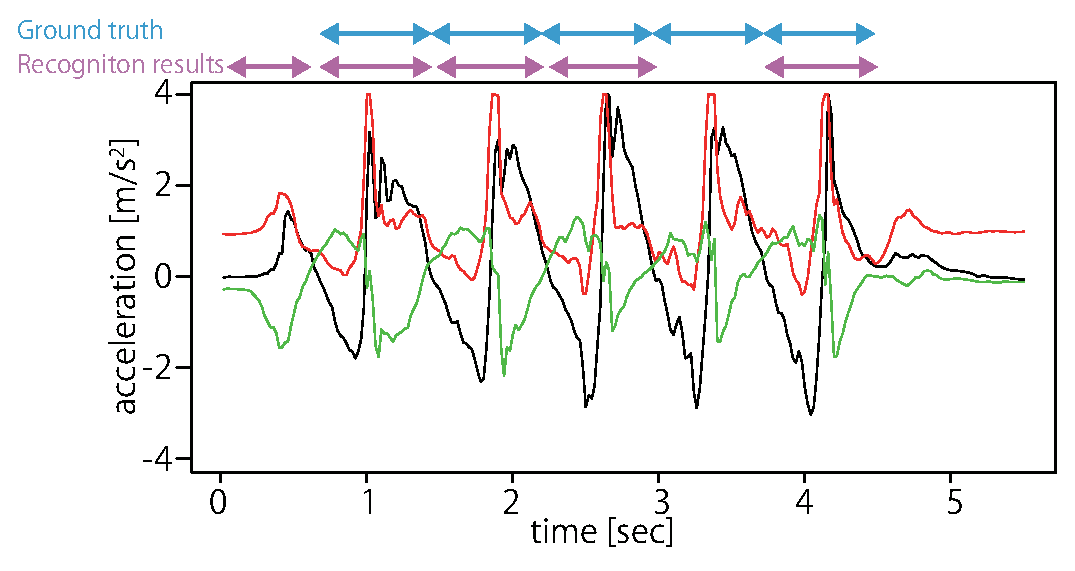
\includegraphics[width=1\linewidth]{images/miss-chop-5x.eps}
            \caption{Acceleration data and results of SPRING for chop gestures performed five times without breaks.}
            \label{fig:miss-chop-5x}
        \end{figure}

        \subsection{Improved SPRING algorithm}
        The classic SPRING algorithm may miss out gestures when same gestures are performed continuously without break. We improve SPRING so that it can output such subsequences separately. Algorithm \ref{fig:spring-improved} shows an algorithm of the improved SPRING. Only line 10 was changed from the classic SPRING. The improved SPRING outputs the subsequence as well if the following condition is met.
        \begin{eqnarray}
            \label{eq:force}
            \forall_{j}, t_s(j) = t_s(t) \cap t_e(j) = t_e(t) \\
            (j = t-\varepsilon_{f}, t-\varepsilon_{f}+1, \dots, t-1) \nonumber
        \end{eqnarray}
        $t_{s}(t)$ and $t_{e}(t)$ are the starting point of the subsequence $t_s$ as of time $t$ and the endpoint of the subsequence $t_e$ as of time $t$. 
        This condition means that the starting point and the endpoint of the subsequence do not change for $\varepsilon_{f}$ samples. $\varepsilon_{f}$ is a predefined number set to 10 samples (200 msec) in this paper.
        
        \begin{algorithm}[!t]
            \begin{algorithmic}[1]
                %\State{\textbf{Algorithm SPRING-improved}}
                \State{\textbf{input}: $X=\{x_1,\dots,x_n$\}
                \State{\textbf{output}: subsequence matching $Y'=\{y_0,y_1,\dots,y_m\}$}}
                \State{$ d_{min} = \infty $}
                \ForTo{$t = 1$}{$n$}
                \ForTo{$i = 0$}{$m$}
                \State{calc. ${\bf d}(t,i)$ with Eqn. \ref{eq:dist-wt}}
                \State{calc. ${\bf s}(t,i)$ with Eqn. \ref{eq:point-wt}}
                \EndFor
                \If{$d_{min} \leq \varepsilon$}
                \If{$\forall_{i}, {\bf d}(t,i) \geq d_{\min} \cup {\bf s}(t,i) > t_{e} \cup $ Eqn. \ref{eq:force}}
                \State{Report$(d_{\min} , t_{s} , t_{e})$}
                \ForTo{$l=1$}{$m$}
                \If{${\bf s}(t,l) \leq t_e $}
                \State{${\bf d}(t,l) = \infty$}
                \EndIf
                \EndFor
                \EndIf
                \EndIf
                \If{${\bf d}(t,m) \leq \varepsilon \cap {\bf d}(t,m) < d_{min}$}
                \State{$d_{min} = {\bf d}(t,m);~t_s={\bf s}(t,m);~t_e=t$}
                \EndIf
                \EndFor
                %\State{Substitute $d'_{i}$ for $d_{i}$}
                %\State{Substitute $s'_{i}$ for $s_{i}$}
            \end{algorithmic}
            \caption{Improved SPRING algorithm.}\label{fig:spring-improved}
        \end{algorithm}
       
       
        \subsection{Gesture recognition algorithm}
        The proposed method detects subsequences of gestures from input stream of acceleration with the improved SPRING and outputs the most likely subsequence as a result of gesture recognition.
        
        %Algorithm \ref{fig:gesture-selection} and Algorithm \ref{fig:gesture-selection2} show the algorithm to output the subsequence that has high likelihood as a result of gesture recognition.
        Figure \ref{fig:gesture-selection-flowchart} shows a flowchart of the procedure to select the most likely subsequence as a result of gesture recognition. The procedure is iterated as the acceleration data is obtained. As input stream of acceleration data comes, the improved SPRING algorithms successively calculate the distance for each template data of target gestures to be recognized and output subsequence if it is found.
        
        \begin{figure}[!t]
            \centering
            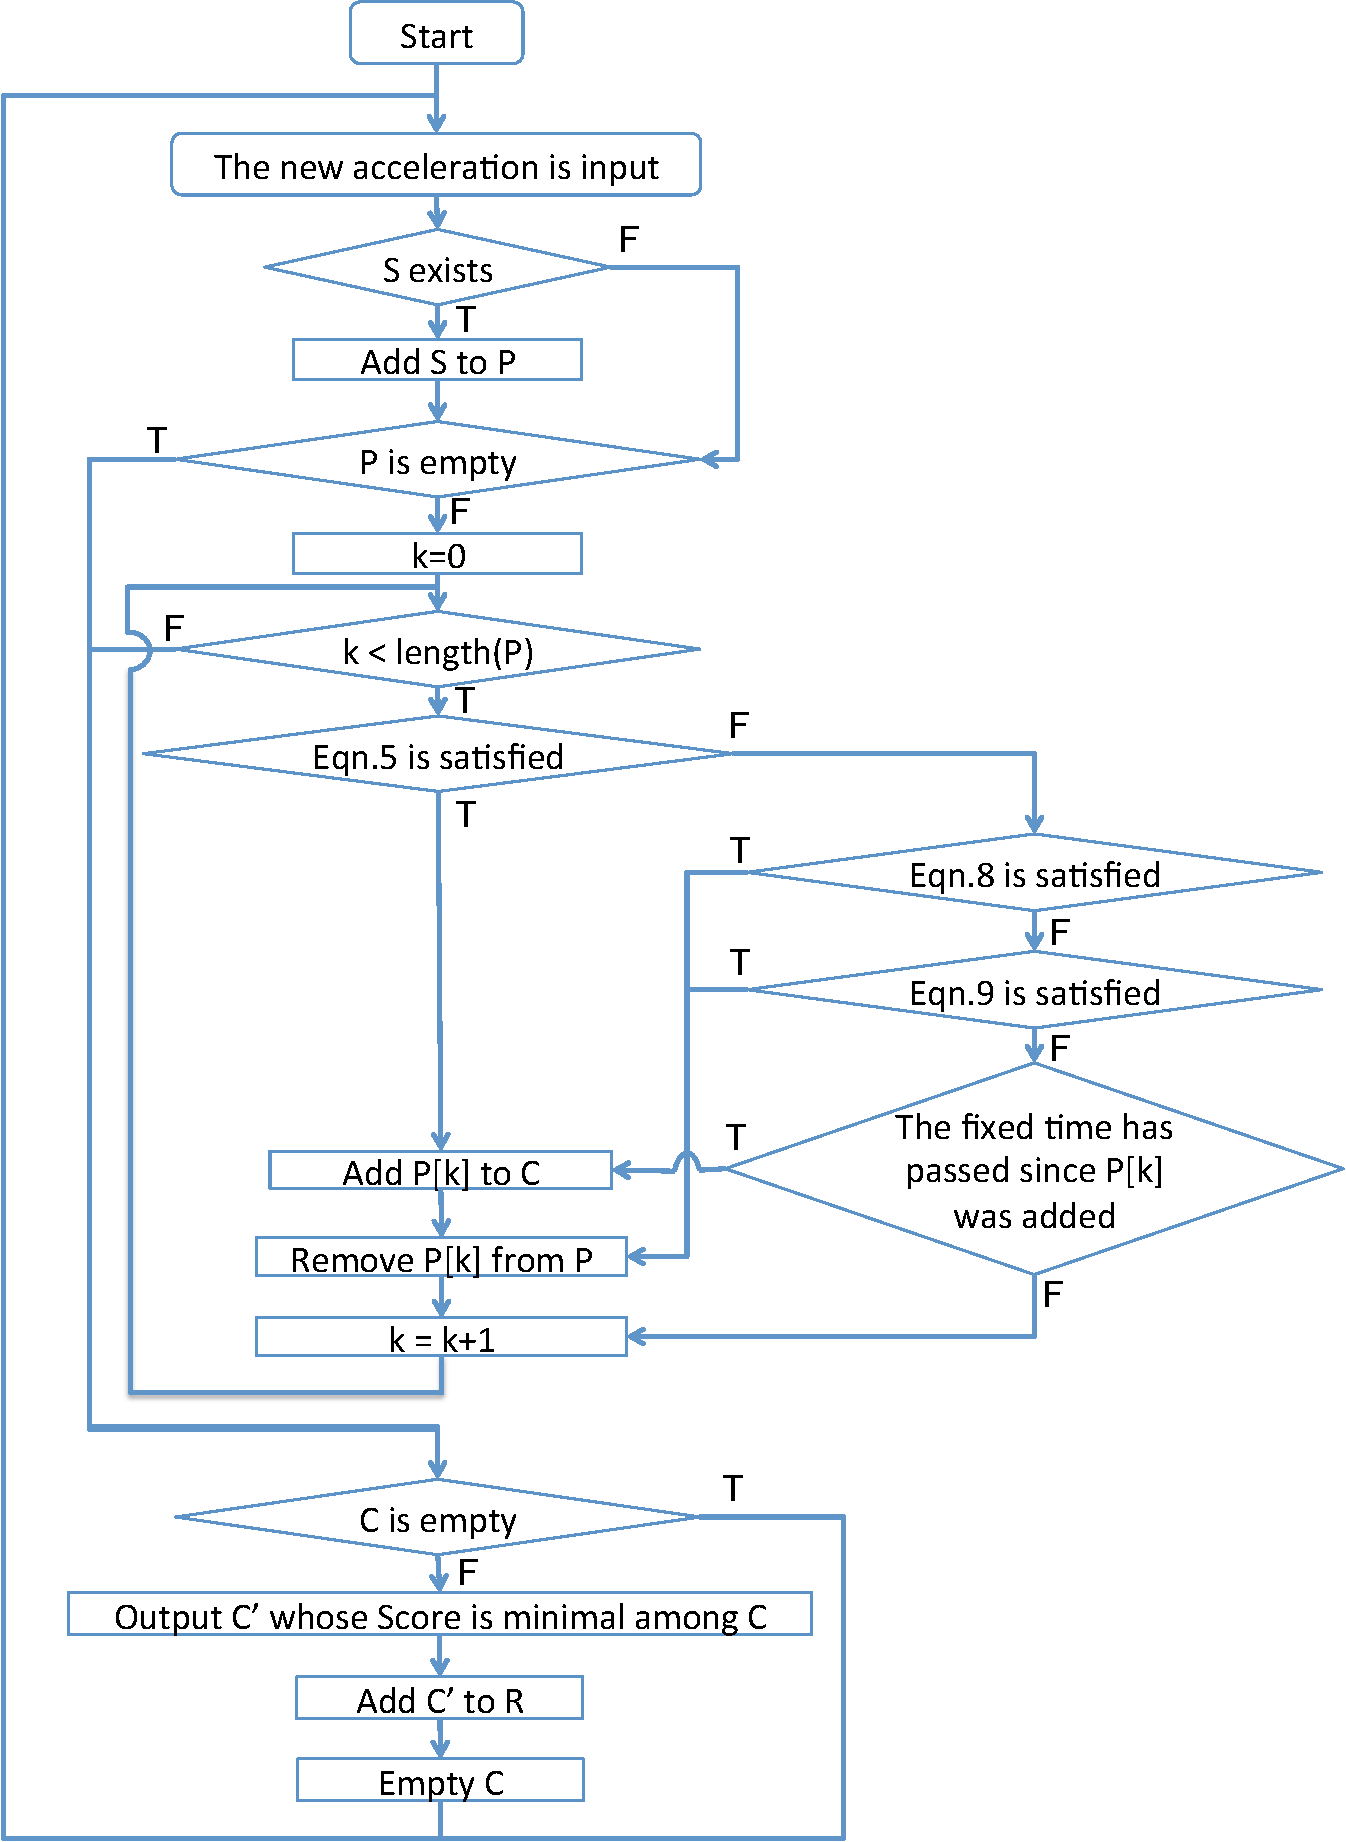
\includegraphics[width=1\linewidth]{images/gesture-detection-flowchart.pdf}
            \caption{Flowchart of gesture recognition algorithm.}
            \label{fig:gesture-selection-flowchart}
        \end{figure}
        
        In the proposed method, the improved SPRING algorithms find a gesture to be recognized in parallel. In short, ten improved SPRING algorithms are running when recognizing ten kinds of gestures with one template data for each. When one of the improved SPRING algorithm finds a subsequence $S$, the proposed method adds $S$ to $P$, which is an array of suspended subsequences. If $P$ is not empty, $P[k]$ is checked for $k=1, \dots, length(P)$ whether the following condition is satisfied, where $length(P)$ is the number of subsequences in $P$, $d_k$ is the distance of $P[k]$, and $d_{\overline{k}}$ is the minimal distance in $P$ other than $P[k]$.
        \begin{eqnarray}
            \label{eq:likelihood}
            \frac{d_k}{d_{\overline{k}}} < \alpha
        \end{eqnarray}
        This condition judges whether $P[k]$ should be output as a result of gesture recognition or not. $\frac{d_k}{d_{\overline{k}}}$ will be smaller value if the difference between $d_k$ and $d_{\overline{k}}$ is larger value, which means that the distance of the gesture which corresponds to $d_k$ is enough smaller than the distances of the other gestures. Therefore, the gesture corresponds to $d_k$ is likely as a result of gesture recognition.
        %the output subsequences do not overlap each other if multiple subsequences are reported from the improved SPRING.
        If Eqn. \ref{eq:likelihood} is satisfied, the proposed method adds $P[k]$ to $C$. $C$ is an array of candidate results of gesture recognition. Then, $P[k]$ is removed from $P$. $ \alpha $ is set to $0.50$ in this paper. 
        
        If Eqn. \ref{eq:likelihood} is not satisfied, the proposed method deletes the suspended subsequence whose likelihood is lower than both the other suspended subsequences and the subsequences that had been output as results. In order to compare likelihood, the proposed method uses Eqn. \ref{eq:duplication-ratio} and Eqn. \ref{eq:dist-s}.
        \begin{eqnarray}
            \label{eq:duplication-ratio}
            D(A,B) =
            \begin{cases}
                \begin{array}{ll}
                    0 & ( A_e < B_s \cup B_e < A_s) \\
                    \frac{B_e - B_s}{A_e - A_s} & ( A_s < B_s \cap B_e < A_e) \\
                    \frac{A_e - B_s}{A_e - A_s} & ( A_s < B_s ) \\
                    \frac{B_e - A_s}{A_e - A_s} & ( A_s > B_s ) \\
                    1 & (otherwise)
                \end{array}
            \end{cases}
        \end{eqnarray}
        \begin{equation}
            \label{eq:dist-s}
            Dist(A) = \frac{d_{min}(A)}{length(A) + length(Y)}
        \end{equation}
        $D(A,B)$ shows the ratio of overlap between the subsequences $A$ and $B$. $A_s$ and $A_e$ are the starting point and endpoint of $A$, respectively. In the same way, $B_s$ and $B_e$ are the starting point and endpoint of $B$, respectively. The range of $D(A,B)$ is from 0 to 1. For example, for the subsequence $A[1:10]$ and $B[6:10]$, Eqn. \ref{eq:duplication-ratio} is $D(A,B) = 0.5$.

        Eqn. \ref{eq:dist-s} is the value to evaluate the likelihood of subsequences. Eqn. \ref{eq:dist-s} shows the distance between the subsequence and the template data corresponding to the subsequence. Eqn. \ref{eq:dist-s} will be smaller value when the likelihood of subsequence is high. In Eqn. \ref{eq:dist-s}, $ d_{min}(A) $ is the minimal value of the distance of the subsequence $A$. $length(A)$ is the length of the subsequence $A$ and $length(Y)$ is the length of a template data $Y$.
        First, the proposed method compares the likelihood of one of pending subsequences with the likelihood of another of pending subsequences, and excludes the one which has a lower likelihood. $P'$ is an array which excluded $P[k]$ from $P$. Then, the proposed method excludes $P[k]$ from $P$ if $p'$ satisfies Eqn. \ref{eq:comarison-pendings}. $p'$ is one of the subsequences $P'$. $M$ is a predefined threshold of the ratio of overlap. It is set to $M=0.33$ in this research. The proposed method repeats this procedure for all of $P$.
        \begin{equation}
            M < D(P[k], p') \cap Dist(p') < Dist(P[k])
            \label{eq:comarison-pendings}
        \end{equation}
        If Eqn. \ref{eq:comarison-pendings} is satisfied, there is a subsequence which has likelihood higher than $P[k]$ and it overlaps with $P[k]$. Therefore, the proposed method excludes $P[k]$ from $P$ because $P[k]$ is not suitable for a result of gesture recognition.

        Next, the proposed method compares the likelihood of one of the pending subsequences with the likelihood of the subsequence which output as a result of gesture recognition, and excludes the subsequence which has lower likelihood than the subsequences were output. $R$ is an array of the subsequences which were output as a result of gesture recognition in the past. Then, $P[k]$ is excluded from $P$ if Eqn. \ref{eq:comarison-results} is satisfied.
        \begin{equation}
            M < D(P[k], r) \cap Dist(r) < Dist(P[k])
            \label{eq:comarison-results}
        \end{equation}
        If Eqn. \ref{eq:comarison-results} is satisfied, a subsequence was output as a result of gesture recognition and it overlaps with $P[k]$. Therefore, the proposed method excludes $P[k]$ from $P$.
        
        Lastly, the proposed method adds $P[k]$ to $C$ as a result of gesture recognition if time $ \varepsilon_t $ has passed since $P[k]$ was added to $P$.
        $ \varepsilon_t $ is a predefined threshold of time. It is set to 25 samples (0.5 sec) in this research. The subsequences which are not suitable as a result of gesture recognition, would be excluded from $P$ by Eqn. \ref{eq:comarison-pendings} and Eqn. \ref{eq:comarison-results}. Therefore if enough time has passed since $P[k]$ was added to $P$, only likely subsequences remain in $P$.
        
        %The subsequence that enough time passed since it was added to $P$ is likely as a result of gesture recognition, because it would be excluded by the procedure of this section if it is not suitable for a result of gesture recognition.

        %The subsequence in $P$ that the predefined time $\varepsilon_t$ has passed since it was added to $P$ will be added to $C$, because if enough time passed since the subsequence added to $P[k]$, $P[k]$ has only the subsequences which has high likelihood by the exclusion explained in this section. Then, the proposed method adds the subsequence 
        %which $\varepsilon_t$ has passed since it was added to $P[k]$, to $C$ as the candidates for a result of gesture recognition.
        %The overview of the proposed method is as follows. First, the proposed method detects the subsequences which similar to template data with the improved SPRING. Next, the proposed method selects the stable one from the detected subsequences because the multiple subsequences detected with the improved SPRING may appear. This selection is based on the rates of overlap and the scores calculated by the distance and the length of subsequences. Finally, the proposed method choose most stable one from the subsequences which detected in previous procedure. % The proposed method repeats as the accelerations are obtained in real time.
        
%        \subsubsection{Selection of the subsequence to output}
        After excluding the subsequences whose likelihood is low, the proposed method decides to output the subsequence. $C$ is the candidates of the subsequence to output. If $C$ is empty, the proposed method skips this procedure and waits until the next acceleration data comes. Otherwise, the proposed method decides to output the subsequence as a result of gesture recognition from $C$.
        If the candidates of subsequence $C$ have only single subsequence, the proposed method outputs one of $C$ as a result of gesture recognition.
        %If the group of the candidates for the result of gesture recognition have multiple subsequences, 
        Otherwise, the proposed method chooses most likely subsequence from $C$. In particular, the proposed method chooses the subsequence $ C' $ whose value of $Dist(C')$ is the minimal value from $C$. $Dist(C')$ is calculated by Eqn. \ref{eq:dist-s}. Then, $C'$ is added to $R$ because it is used for the comparison on Eqn. \ref{eq:comarison-results}.
        After that, the proposed method empties $C$ and waits until next acceleration data comes.

        \section{Evaluation}
        \subsection{Setup}
        In order to evaluate the effectiveness of the proposed method, we conducted an experiment with five subjects who attached an accelerometer on their right wrist. The accelerometer used in the experiment is TSND121 manufactured by ATR-Promotions, Inc. The frequency is set to 50 Hz. The subjects conducted three types of gestures drawing a graphic symbol in the air: circle, triangle, and cross in five kinds of situations shown Table \ref{tab:gesture-pattern}. The untrained activity in Table \ref{tab:gesture-pattern} is waving hands as though walking. Each subject performed the pattern once.
        In addition, the subjects conducted ten types of gestures drawing a numeric character in the air: zero to nine. As an evaluation index, F-measure of gesture recognition is calculated from a result of the experiment with Eqn. \ref{eq:precision}.
        \begin{eqnarray}
            \label{eq:precision}
            Precision & = & \frac{\mbox{\# of gestures recognized correctly}}{\mbox{\# of gestures performed actually}} \nonumber \\
            Recall    & = & \frac{\mbox{\# of gestures recognized correctly}}{\mbox{\# of output gestures}} \nonumber \\
            F-Measure & = & \frac{2 \cdot Precision \cdot Recall}{Precision+Recall} \nonumber 
        \end{eqnarray}
        
        \begin{table}[!t]
            \centering
            \caption{List of patterns of gestures drawing a graphic symbol.}
            \label{tab:gesture-pattern}
            \begin{tabular}{c|l}\hline\hline
                Pattern & Detail of activity \\ \hline
                1 & Circle 5 times \\
                2 & Triangle 5 times  \\
                3 & Cross 5 times \\
                4 & Circle and Triangle 5 times continuously \\
                5 & Circle and Cross 5 times continuously \\
                6 & Triangle and Cross 5 times continuously \\
                7 & Circle before untrained activity \\
                8 & Triangle before untrained activity \\
                9 & Cross before untrained activity \\
                10 & Circle after untrained activity \\
                11 & Triangle after untrained activity \\
                12 & Cross after untrained activity \\
                13 & Circle during untrained activity \\
                14 & Triangle during untrained activity \\
                15 & Cross during untrained activity \\\hline
            \end{tabular}
        \end{table}
        
        \subsection{Results and consideration}\label{sec:symbol}
        Table \ref{tab:result} shows F-measures for gestures drawing a graphic symbol with 15 patterns in Table \ref{tab:gesture-pattern}. The overall average F-measures is 0.78. On the pattern 11 of subject A and pattern 15 of subjects D and E, F-measures were zero. This is because untrained activities were recognized as gestures and the performed gesture was not recognized as a gesture.

        \begin{table}[!t]
        \centering
            \caption{F-measures for gestures drawing a graphic symbol.}
            \label{tab:result}
            \begin{tabular}{c|ccccc}\hline\hline
                Pattern & A & B & C & D & E \\ \hline
                1  & 1.00  & 1.00 & 0.91 & 0.91 & 0.91 \\
                2  & 0.80  & 0.91 & 0.91 & 1.00 & 0.80 \\
                3  & 0.50  & 0.75 & 0.80 & 0.75 & 0.75 \\
                4  & 0.89  & 0.67 & 0.84 & 0.80 & 0.78 \\
                5  & 0.78  & 0.90 & 0.95 & 0.91 & 0.74 \\
                6  & 0.63  & 0.56 & 0.67 & 0.95 & 0.86 \\
                7  & 1.00  & 1.00 & 1.00 & 0.00 & 0.50 \\
                8  & 0.50  & 1.00 & 1.00 & 1.00 & 1.00 \\
                9  & 0.40  & 1.00 & 0.67 & 0.00 & 1.00 \\
                10 & 1.00  & 0.67 & 1.00 & 1.00 & 1.00 \\
                11 & 0.00  & 0.67 & 1.00 & 1.00 & 1.00 \\
                12 & 0.33  & 1.00 & 1.00 & 1.00 & 1.00 \\
                13 & 1.00  & 1.00 & 1.00 & 1.00 & 1.00 \\
                14 & 0.25  & 1.00 & 0.50 & 1.00 & 0.67 \\
                15 & 0.40  & 1.00 & 1.00 & 0.00 & 0.00 \\\hline
            \end{tabular}
        \end{table}

        Table \ref{tab:num-result} shows F-measures for gestures drawing a numeric character. The overall average F-measures is 0.79. F-measure for drawing zero five times by subject A is 0.36 and drawing six five times by subject D is 0.46. This is because six has a part similar to zero. 

        \begin{table}[!t]
        \centering
            \caption{F-measures for gestures drawing a numeric characters.}
            \label{tab:num-result}
                \begin{tabular}{c|cc}\hline\hline
                    Pattern & Subject & F-measure \\ \hline
                    Zero 5 times& A & 0.36  \\
                    One 5 times& A & 0.80  \\
                    Two 5 times& B & 0.89  \\
                    Three 5 times & B & 1.00  \\
                    Four 5 times& C & 0.91  \\
                    Five 5 times & C & 1.00  \\
                    Six 5 times& D & 0.46  \\
                    Seven 5 times & D & 0.80  \\
                    Eight 5 times& E & 0.67  \\
                    Nine 5 times& E & 0.55  \\ \hline
                    & A & 1.00  \\
                    & B & 0.87  \\
                    Zero to Nine sequentially & C  & 0.90  \\
                    & D & 0.76  \\
                    & E & 0.84  \\\hline
                \end{tabular}
        \end{table}

        \section{Conclusion}
        We proposed a method that recognizes gestures performed continuously from/to other gestures or untrained activities. An algorithm to detect the subsequence that has lower distance to a query of time-series than the predefined threshold from a time-series data called SPRING has been proposed, however, SPRING may miss consecutive gestures. Therefore, we improved SPRING and used it to detect the segment of gestures. The proposed method detects the segment similar to template data as a subsequence and outputs the most likely subsequence as a result of gesture recognition. In the experiment, gestures drawing a graphic symbol and a numeric character were recognized with 0.78 F-measure and 0.79 F-measure, respectively.

%        Our system uses only the minimal distance to choose the suitable subsequence from the subsequences detected by SPRING. However, it is considerable to use other values such as the distance with template data of other gestures.

        The output of the proposed method has a small delay since the proposed method suspends the output for a while in order to see if other gestures are also detected. In the future, we plan to improve the method to output the results before the gestures end.
        
        \section*{Acknowledgments}
        This research was supported in part by a Grant-in-Aid of the Kayamori Foundation of Information Science Advancement.

        \newpage

        \bibliographystyle{SIGCHI-Reference-Format}
        %\bibliography{sample}
        \begin{thebibliography}{99}
            \bibitem{izuta} R. Izuta, K. Murao, T. Terada, M, Tsukamoto. Early Gesture Recognition Method with an accelerometer. International Journal of Pervasive Computing and Communications, Vol. 11, No, 6, pp 270--287 (Apr. 2015).
            \bibitem{uwave} J. Liu, L. Zhong, J. Wickramasuriya, V. Vasudevan. uWave: Accelerometer-based personalized
            gesture recognition and its applications. In proc. of International Conference
            on Pervasive and Mobile Computing (PerCom 2009), Vol. 5, No. 6, pp. 657--675 (Mar.
            2009).
            \bibitem{dtw} C.S. Myers, L.R. Rabiner. A comparative study of several dynamic time-warping algorithms
            for connected-word recognition. The Bell System Technical Journal, Vol. 60,
            No. 7, pp. 1389--1409 (Sep. 1981).
            \bibitem{hmm} L.R. Rabiner, B.H. Juang, A tutorial on hidden markov models and selected applications in speech recognition, IEEE, pp 257--286 (1989).
            \bibitem{murao-const} K. Murao and T. Terada. A Motion Recognition Method by Constancy-Decision, in Proc. of IEEE International Symposium on Wearable Computers (ISWC 2010), pp. 69--72, Seoul, Korea (Oct. 2010).
            \bibitem{murao-comb} K. Murao, T. Terada. A Combined-Activity Recognition Method with Accelerometers, Journal of Information Processing Society of Japan, Vol. 24, No. 3, pp. 512--521 (May 2016).
            \bibitem{joseph} J. Korpela, K. Takase, T. Hirashima, T. Maekawa, J. Eberle, D. Chakraborty, K. Aberer. An energy-aware method for the joint recognition of activities and gestures using wearable sensors. In proc. of the 2015 ACM International Symposium on Wearable Computers (ISWC  2015), pp. 101--108 (Sep. 2015).
            \bibitem{park} T. Park, J. Lee, I. Hwang, C. Yoo, L. Nachman, J. Song. E-Gesture: a collaborative architecture for energy-efficient gesture recognition with hand-worn sensor and mobile devices. In proc. of the 9th ACM Conference on Embedded Networked Sensor Systems (SenSys 2011), pp. 260--273 (Nov. 2011).
            \bibitem{sakurai} Y. Sakurai. C, Faloutsos, M. Yamamuro. Stream
            Monitoring under the Time Warping Distance.  In proc. of the IEEE 23rd
            International Conference on Data Engineering (ICDE 2007), pp. 1046--1055 (Apr. 2007).
        \end{thebibliography}
    \end{document}

    %%% Local Variables:
    %%% mode: latex
    %%% TeX-master: t
    %%% End:
